\documentclass[11pt,a4paper]{article}

%==============================================================================%

\usepackage{a4wide}
\usepackage{amsmath,amssymb}
\usepackage[utf8]{inputenc}
\usepackage{float}
\usepackage{graphicx}
\usepackage{listings}
\usepackage{multicol}
\usepackage{tikz}

\usetikzlibrary{arrows}

%==============================================================================%

\newcommand{\assignmentnumber}{3}

\newcommand{\modulus}[1]{\lvert#1\rvert}
\newcommand{\conjugate}[1]{\bar{#1}}
\newcommand{\degree}{^{\circ}}
\newcommand{\limit}[2]{\lim_{#1 \rightarrow #2}}

\newcommand{\figref}[1]{fig. \ref{fig:#1}}
\newcommand{\eqnref}[1]{(\ref{eqn:#1})}

\DeclareMathOperator{\re}{Re}
\DeclareMathOperator{\im}{Im}

\renewcommand\thesection{\assignmentnumber.\arabic{section}}
\renewcommand\thesubsection{\alph{subsection})}

%==============================================================================%

\title{MatIntro Pointopgave \assignmentnumber}
\author
{
    Casper B. Hansen\\
    University of Copenhagen\\
    {\tt fvx507@alumni.ku.dk}
}
\date{\today}

%==============================================================================%

\begin{document}

% \maketitle


% 3.1
\section
{
    \mdseries
    Lad $f(x) = \frac{1}{x} - \frac{\cos x}{\sin x}$ for alle $x \in
    \mathbb{R}$ med $x \neq n\pi, n \in \mathbb{Z}$.
}
Til følgende opgaver defineres følgende erklæres følgende udsagn i Maple.
\begin{lstlisting}
    f := x -> (1/x) - cos(x)/sin(x)
\end{lstlisting}

% 3.1 (a)
\subsection
{
    \mdseries
    Find grænseværdierne $\limit{x}{0+} f(x)$, $\limit{x}{\pi-} f(x)$ først
    med og dernæst uden Maple.
}
I Maple skriver vi følgende og får resultaterne $0$ hhv. $\frac{1}{\pi} -
\frac{\cos \pi}{\sin \pi}$.
\begin{lstlisting}
    limit(f(x), x=0, right);
    limit(f(x), x=pi, left);
\end{lstlisting}

\begin{multicols}{2}

    \noindent
    Ved håndregning af $\limit{x}{0^+} f(x)$ omformulerer vi
    \begin{align}
        \limit{x}{0^+} \left( \frac{1}{x} - \frac{\cos x}{\sin x} \right)
        &= \limit{x}{0^+} \left( \frac{\sin x - x \cos x}{x \sin x} \right)
        \label{eqn:3.1a-1}
    \end{align}

    Vi kan se, at \eqnref{3.1a-1} er et $\frac{0}{0}$-udtryk, når $x
    \rightarrow 0+$, og benytter derfor L'Hôpital's regel, indtil vi har en
    grænseværdi, der giver mening.

    \begin{align}
        &\limit{x}{0^+} \left( \frac{\sin x - x \cos x}{x \sin x} \right) \\
        &= \limit{x}{0^+} \left( \frac{x \sin x}{\sin x + x \cos x} \right) \\
        &= \limit{x}{0^+} \left( \frac{\sin x + x \cos x}{2 \cos x - \sin x} \right)
         = \frac{0}{2} = 0
    \end{align}
    
    Altså, er $\limit{x}{0^+} \left( \frac{1}{x} - \frac{\cos x}{\sin x}
    \right) = 0$.
    
    \vfill{\ }\columnbreak

    \noindent
    For $\limit{x}{\pi^-} f(x)$ har igen vi, at
    \begin{align}
        \limit{x}{\pi^-} \left( \frac{1}{x} - \frac{\cos x}{\sin x} \right)
        &= \limit{x}{\pi^-} \left( \frac{\sin x - x \cos x}{x \sin x} \right)
    \end{align}
    
    Vi bemærker at $\limit{x}{\pi^-} x \sin x = 0$, medens $\limit{x}{\pi^-}
    \sin x - x \cos x = -\pi(-1) = \pi$. Nævneren er altså $0$ i $x = \pi$,
    men da $\sin x > 0$, $\forall x \in (2n\pi, (2n+1)\pi)$, hvor $n \in
    \mathbb{Z}$ ved vi, at $\frac{\sin x - x \cos x}{x \sin x} > 0$, $\forall
    x \in (2n\pi,(2n+1)\pi)$, hvor $n \in \mathbb{Z}$. Nævneren bliver altså
    meget lille, men er fortsat positiv. Derfor har vi at
    \begin{align}
        \limit{x}{\pi^-} \left( \frac{\sin x - x \cos x}{x \sin x} \right) &= \infty
    \end{align}
    \vfill{\ }

\end{multicols}

% 3.1 (b)
\subsection
{
    \mdseries
    Vis, at $f$ er strengt voksende i hvert interval $(n\pi,(n+1)\pi)$.
    Uligheden $\modulus{\sin x} < \modulus{x}$ for $x \neq 0$ kan benyttes
    uden bevis (den er vist i TLO side 240).
}
\label{sec:3|sub:1|ass:b}
Lad os først differentiere $f$, da denne vil give os mulighed for at
undersøge væksten af funktionen.
\begin{align}
    f'(x) &= \left( \frac{1}{x} \right)'
           - \left( \frac{\cos x}{\sin x} \right)'
           = \frac{\cos(x)^2}{\sin(x)^2} - \frac{1}{x^2} + 1
\end{align}

Konstanten kan vi ignorere. Vi bemærker at de nævnerne i de øvrige led er
kvadrerede, og dermed altid positive. For at $f$ kan vises at være strengt
voksende i intervallet, må vi da vise, at $\frac{\cos(x)^2}{\sin(x)^2} >
\frac{1}{x^2}$. Siden $\modulus{\sin x} < \modulus{x}$ og $0 \leq \cos(x)^2
\leq 1$ holder dette udsagn. I tilfældet, hvor $x = n\pi$, hvor $n \in
\mathbb{Z}$, er funktionen ikke defineret pga. division med nul og ekskluderes
derfor fra $D_f$. Uligheden holder derfor kun i $x \in (n\pi, (n+1)\pi)$, $n
\in \mathbb{Z}$.

Vi har altså, at
\begin{align}
    f'(x) &= \frac{\cos(x)^2}{\sin(x)^2} - \frac{1}{x^2} + 1 > 0
          , \forall x \in (n\pi, (n+1)\pi)
\end{align}

% 3.1 (c)
\subsection
{
    \mdseries
    Bevis, at ligningen $f(x) = 0$ ikke har nogen løsninger i $(0, \pi)$, og
    at den har præcis én løsning i $(\pi,2\pi)$. Benyt Maple til at finde en
    approksimering til denne løsning.
}
Siden vi ved, at $f$ er strengt voksende (se opgave 3.1\ref{sec:3|sub:1|ass:b})
i $(n\pi,(n+1)\pi)$ og at $\limit{x}{0+} f(x) = 0$ gælder, at $0 < f(x)$,
$\forall x \in (n\pi,(n+1)\pi)$. Hvis vi lader $n=0$ har vi, at $0 < f(x)$,
$\forall x \in (0,\pi)$ og dermed også $f(x) \neq 0$, $\forall x \in (0,\pi)$
--- ligningen $f(x) = 0$ har altså ingen løsninger i $(0,\pi)$.

Igen, idet vi ved at $f$ er strengt voksende i intervaller $(n\pi,(n+1)\pi)$,
skal vi blot argumentere at $\limit{x}{\pi+} f(x) < 0 < \limit{x}{2\pi-}$,
hvilket ville medføre, at $f$ nødvendigvis må skære $x$-aksen i intervallet.

I opgave (a) dragede vi følgende udsagn; $\sin x > 0$, $\forall x \in (2n\pi,
(2n+1)\pi)$. Tilsvarende gælder det, at $\sin x < 0$, $\forall x \in ((2n+1)\pi,
2n\pi)$, derfor har vi, at

\begin{align}
    \limit{x}{\pi^+} \left( \frac{\sin x - x \cos x}{x \sin x} \right)
    &= -\limit{x}{\pi^-} \left( \frac{\sin x - x \cos x}{x \sin x} \right)
     = -\infty
\end{align}

Ligeledes, observerer vi, at $\sin(2\pi) = \sin(\pi)$ og $\cos(2\pi) = -\cos
\pi$. Dette minder meget om $\limit{x}{\pi^-} f(x)$, men vi skal huske at
vende fortegnet, da det nu gælder at $\sin x < 0$ i intervallet, som påvist
tidligere. Altså, idet $\cos(2\pi) = -\cos \pi$, skal vi vende fortegnet, men
siden $\sin x < 0$ i intervallet, skal vi igen vende det. Vi har derfor, at

\begin{align}
    \limit{x}{2 \pi^-} \left( \frac{\sin x - x \cos x}{x \sin x} \right)
    &= \limit{x}{\pi^-} \left( \frac{\sin x - x \cos x}{x \sin x} \right)
     = \infty
\end{align}

Ud fra dette, kan vi slutte, at $\limit{x}{\pi^+} < 0 < \limit{x}{2\pi^-}$,
og siden $f(a) < f(b)$, $\forall a < b \in (\pi, 2\pi)$ ved vi, at der
findes en og kun én løsning til ligningen $f(x) = 0$ i $x \in (\pi, 2\pi)$.

I Maple finder jeg approksimeringen af $f(x) = 0$, $x \in (\pi,2\pi)$ ved
\begin{lstlisting}
fsolve(f(x)=0,x=Pi..2Pi)
\end{lstlisting}
hvilket giver mig en approksimation på $x \approx 4.493409457909064175308$

% 3.2
\section
{
    \mdseries
    En funktion $f : \mathbb{R} \rightarrow \mathbb{R}$ defineres ved
    \eqnref{3.2}
}
\begin{align}
    f(x) &=
    \begin{cases}
        \frac{1 - x^2}{(x -1)(x - 3)} &x \in (-\infty;1) \cup (3;\infty) \\
        x &x \in [1;3]
    \end{cases}
    \label{eqn:3.2}
\end{align}

I Maple har jeg erklæret funktionen, som følger
\begin{lstlisting}
c1 := x -> x < 1 or x > 3
c2 := x -> 1 <= x <= 3

f1 := x -> (1 - x^2) / ((x - 1)(x - 3))
f2 := x -> x

f  := x -> piecewise(c1(x), f1(x), c2(x), f2(x))
\end{lstlisting}

\begin{multicols}{2}
    % 3.2 (a)
    \subsection
    {
        \mdseries
        Lav i Maple et plot af et udsnit af grafen for $f$, der giver et
        retvisende og oplysende billede af funktionens overordnede opførsel.
    }

    \begin{figure}[H]
        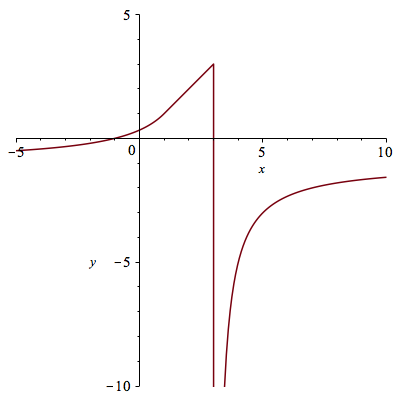
\includegraphics[scale=0.5]{figures/3-2a-1.png}
        \caption{Grafen for $f$ i intervallet $x,y \in [-5,10]$}
        \label{fig:3.2a-1}
    \end{figure}

    \vfill{\ }\columnbreak

    % 3.2 (b)
    \subsection
    {
        \mdseries
        Er $f$ differentiabel i $x=1$? Begrund dit svar uden brug af Maple.
    }
    Ja. Vi ved, at
    \begin{align}
        \limit{x}{a-} f(x) = \limit{x}{a+} f(x)
        &\implies
        \exists \limit{x}{a} f(x)
    \end{align}

    Det er let at se, at $\limit{x}{1+} f(x) = 1$, så lad os kigge på den
    anden side.
    
    Vi ser, at $\frac{1 - x^2}{(x - 1)(x - 3)}$ giver et $\frac{0}{0}$-udtryk
    for $x = 1$. Derfor ganger vi først ud, for at gøre det nemmere
    \begin{align}
        \frac{1 - x^2}{(x - 1)(x - 3)} &= \frac{1 - x^2}{x^2 - 4x + 3}
    \end{align}
    og benytter os derefter af L'Hôpitals regel.
    \begin{align}
        \limit{x}{1-} \frac{1 - x^2}{x^2 - 4x + 3} &=
        \limit{x}{1-} \frac{-2x}{2x - 4} = 1
    \end{align}

    Da $\limit{x}{1-} f(x) = \limit{x}{1+} = 1$, har vi at
    \begin{align}
        \limit{x}{1} f(x) = 1
    \end{align}

    Og funktionen $f$ er derfor differentiabel i $x = 1$.

    \vfill{\ }

\end{multicols}


% 3.3 (iii)
\section
{
    (iii) \mdseries
    Betragt funktionen $f(x) = x(\ln(x + 1) - \ln x), x > 0$.
}

% 3.3 (iii) (a)
\subsection
{
    \mdseries
    Tegn grafen for $0 < x \leq 100$ og gæt på $\limit{x}{\infty} f(x)$ ud
    fra denne.
}
\begin{multicols}{2}
    Funktionen defineres og plottes i Maple som
\begin{lstlisting}
f := x -> x (ln(x + 1) - ln(x))

plot(f(x), x=0..100)
\end{lstlisting}
    
    Mit umiddelbare gæt er, at funktionen er asymptote med $y = 1$, og derfor
    at $\limit{x}{\infty} f(x) = 1$.

    \vfill{\ }\columnbreak

    \begin{figure}[H]
        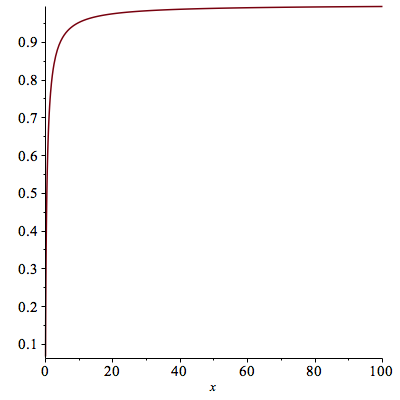
\includegraphics[scale=0.5]{figures/3-3(iii)a-1.png}
        \caption{Grafen for $f$ i intervallet $x \in [0,100]$}
        \label{fig:3.3(iii)a-1}
    \end{figure}

\end{multicols}


% 3.3 (iii) (b)
\subsection
{
    \mdseries
    Beregn i Maple $f(10^n)$ for $n = 1, \dots, 10$ (brug f. eks. værdien 20
    af Digits=antal decimaler). Gæt igen på $\limit{x}{\infty} f(x)$ ud fra
    disse tal.
}
\begin{multicols}{2}
    
    I Maple angiver jeg
\begin{lstlisting}
Digits := 22

evalf(f(10^1))
evalf(f(10^2))
evalf(f(10^3))
evalf(f(10^4))
evalf(f(10^5))
evalf(f(10^6))
evalf(f(10^7))
evalf(f(10^8))
evalf(f(10^9))
evalf(f(10^10))
\end{lstlisting}

    \vfill{\ }\columnbreak

    Og får følgende resultater;
    \begin{align}
        f(10^1)     &= 0.953100179804324860044 \\
        f(10^2)     &= 0.9950330853168082848 \\
        f(10^3)     &= 0.999500333083533167 \\
        f(10^4)     &= 0.99995000333308335 \\
        f(10^5)     &= 0.999995000033333 \\
        f(10^6)     &= 0.99999950000033 \\
        f(10^7)     &= 0.99999995000000 \\
        f(10^8)     &= 0.99999999500000 \\
        f(10^9)     &= 0.99999999950000 \\
        f(10^{10})  &= 0.99999999995000
    \end{align}

\end{multicols}

Hvilket stemmer meget godt overens med mit første gæt, og mit er derfor
uændret, ud fra disse resultater.

% 3.3 (iii) (c)
\subsection
{
    \mdseries
    Bestem $\limit{x}{\infty} f(x)$ uden brug af Maple. Kommenter resultaterne
    fra (a) og (b).
}
Vi starter med at omformulere udtrykket
\begin{align}
    \limit{x}{\infty} f(x)
    &= \limit{x}{\infty} x \left( \ln(x + 1) - \ln(x) \right)
     = \limit{x}{\infty} x \cdot \ln \left( \frac{x + 1}{x} \right) \\
    &= \limit{x}{\infty} x \cdot \ln \left( 1 + \frac{1}{x} \right)
     = \limit{x}{\infty} \frac{ \ln \left( 1 + \frac{1}{x} \right) }{1 / x}
\end{align}

Vi bemærker nu at $\limit{x}{\infty} \ln \left( 1 + \frac{1}{x} \right) = 0$,
da som $\limit{x}{\infty} \frac{1}{x} = 0$ og $\ln 1 = 0$. Ligeledes, går
nævneren imod $0$ når $x \rightarrow \infty$. Vi har derfor et
$\frac{0}{0}$-udtryk, og anvender derfor L'Hôpitals regel;
\begin{align}
    \frac{\limit{x}{\infty} \ln \left( 1 + \frac{1}{x} \right) }
         {\limit{x}{\infty} (1 / x)}
    &= \frac{\limit{x}{\infty} \ln \left( 1 + \frac{1}{x} \right)' }
            {\limit{x}{\infty} (1 / x)'}
     = \limit{x}{\infty}
       \frac{ \frac{1}{1 + 1/x} \cdot \left( -\frac{1}{x^2} \right) }{-1 / x^2}
     = \limit{x}{\infty}
       \frac{1}{1 + 1/x}
     = \frac{1}{1} = 1
\end{align}

\end{document}
